\section{Introduction}

Stepper that can display all immediate states of a program is a useful tool for debugging and education. It simplifies expression step by step so that people can track the evaluation procedure easily. \Hazel, a programming language environment developed by [citation Cyrus Omar], allows to evaluate incomplete programs. It defines a special variable called hole indicating the place that needs to fill. In this paper, we want to develop an interactive stepper for \Hazel. Take the following programs as examples:

\begin{figure}[htbp]
  \centering
  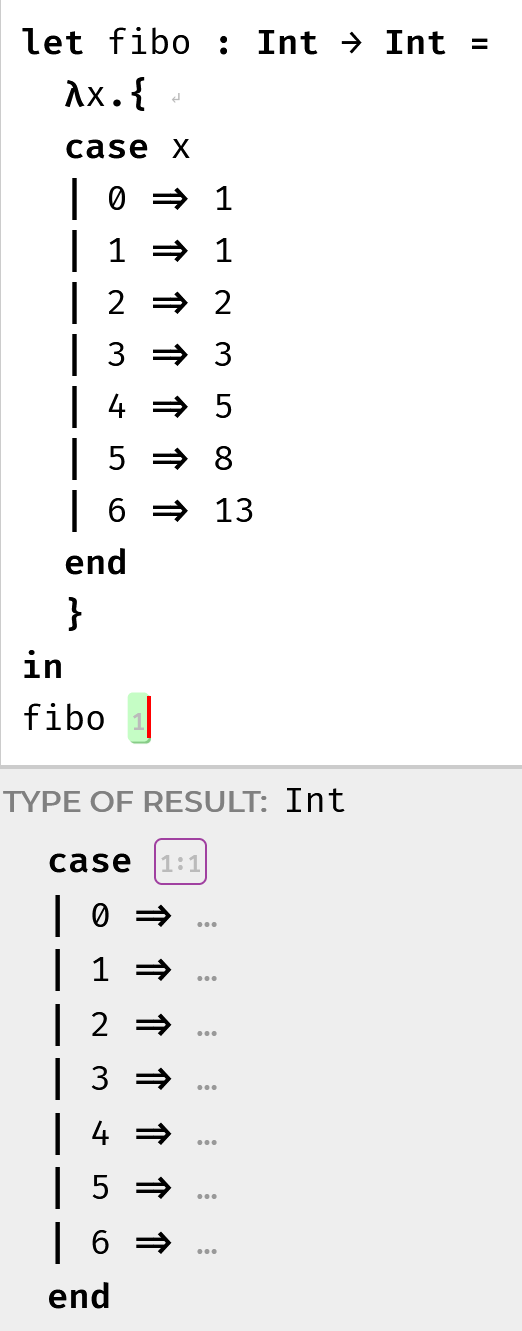
\includegraphics[width=0.5\textwidth]{img/pause_example.png}
  \caption{Example of Paused Environment}
  \label{fig:pause}
\end{figure}

\begin{figure}[htbp]
  \centering
  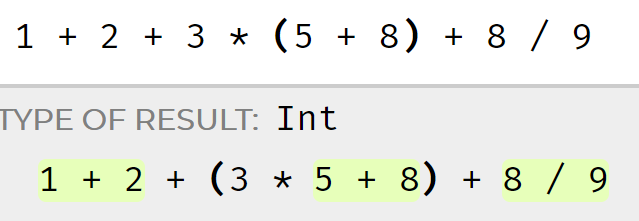
\includegraphics[width=0.5\textwidth]{img/multi_evaluation.png}
  \caption{Example of Multiple Environment}
  \label{fig:multiple}
\end{figure}

% Findler et al.[citation] developed a stepper for DrScheme in their programming environment. Cong and Asai [citation] used the contextual dynamics to build a stepper, which takes subexpression out and plug in after evaluation. In this paper, we will use the similar strategy to develop the stepper. 

In Hazel , the incomplete programs are also allowed for evaluation.  There are two examples shown in Figure \ref{fig:multiple}.



In the first example, the expression is already simple enough and it is unnecessary to expand cases since the parameter has not provided. Therefore, stepper need to detect this situation so that it will pause until user requires it to progress. Another example has an expression with two parts. The left part is heavy since it takes about 16 steps to final while user might just want to debug the right part. According to the regular dynamics, there should contain only one way to step for any non-final programs. So, user has to click 16 times to reduce the left one in order to debug the right one. The possible solution is just allowing the multiple evaluation contexts so that user can choose the subexpression they need. This paper develops a stepper with multiple evaluation contexts and pausing environment.